\documentclass{standalone}
\usepackage{tikz}

%% Document
\begin{document}
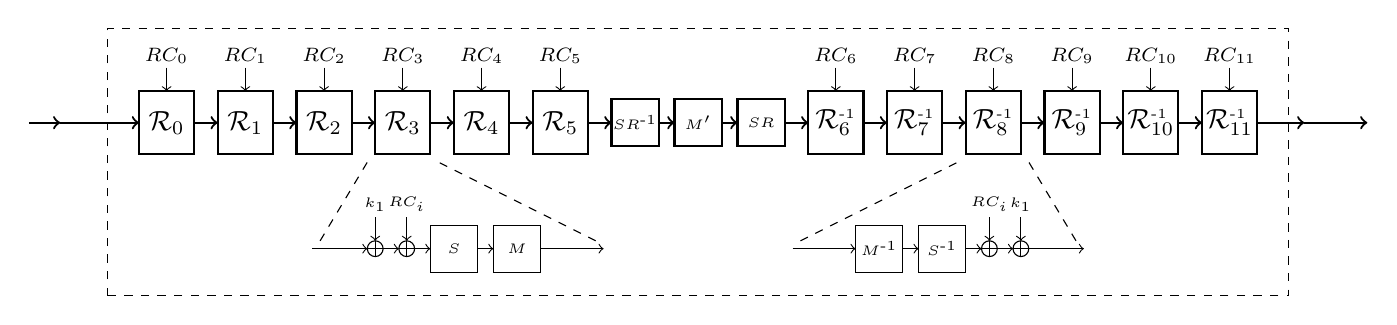
\begin{tikzpicture}[scale=0.20]

\draw[->,thick] (-7,2) -- ++(2,0);
\draw[->,thick] (-5,2) -- ++(5,0);

    \foreach \x in {0,...,5} {
        \def \z{5*\x}
        \draw[thick] (\z,0) rectangle node[]{$\mathcal{R}_{\x}$} ++(3.5,4);
        \draw[->,thick] (\z+3.5,2) -- ++(1.5,0);
        \draw[->] (\z+1.75,5.5) -- ++(0,-1.5);
        \draw[] (\z+1.75,6.25) node[]{\scriptsize $RC_{\x}$} ++(0,0);
    }

    \def \z{5*6}
    \draw[thick] (\z,0.5) rectangle node[]{\tiny $SR^{\textnormal{\tiny -1}}$} ++(3,3);
    \draw[->,thick] (\z+3,2) -- ++(1,0);
    \def \z{5*6+4}
    \draw[thick] (\z,0.5) rectangle node[]{\tiny $M'$} ++(3,3);
    \draw[->,thick] (\z+3,2) -- ++(1,0);
    \def \z{5*6+8}
    \draw[thick] (\z,0.5) rectangle node[]{\tiny $SR$} ++(3,3);

    \foreach \x in {6,...,11} {
        \def \z{5*6+12.5+5*\x - 5*6}
        \draw[->,thick] (\z+3.5-5,2) -- ++(1.5,0);
        \draw[thick] (\z,0) rectangle node[]{$\mathcal{R}^{\textnormal{\tiny -1}}_{\x}$} ++(3.5,4);
        \draw[->] (\z+1.75,5.5) -- ++(0,-1.5);
        \draw[] (\z+1.75,6.25) node[]{\scriptsize $RC_{\x}$} ++(0,0);
    }

    \def \z{5*6+12.5+5*12 - 5*6}
    \draw[->,thick] (\z+3.5-5,2) -- ++(3,0);
    \draw[->,thick] (\z+6.5-5,2) -- ++(4,0);

    \draw[style=dashed] (-2,-9) rectangle ++(5*6+12.5+5*12 - 5*6 +2.5 ,17);
%    \draw[] (5*6+4+1.5 ,8.5) node[above]{$\texttt{PRINCE}_{core}$} ++(0,0);

%    \draw[thick] (-4,2) circle (1);
%    \draw[thick] (-4,3) -- ++(0,-2);
%    \draw[->,thick] (-4,6) -- ++(0,-3);
%    \draw[] (-4,6) node[above]{$k_0$} ++(0,0);
%    \draw[thick] (5*6+12.5+5*12 - 5*6 +2.5,2) circle (1);
%    \draw[thick] (5*6+12.5+5*12 - 5*6 +2.5,3) -- ++(0,-2);
%    \draw[->,thick] (5*6+12.5+5*12 - 5*6 +2.5,6) -- ++(0,-3);
%    \draw[] (5*6+12.5+5*12 - 5*6 +2.5,6) node[above]{$k'_0$} ++(0,0);

    \def \z{5*3}
    \draw[->] (\z-4,-6) -- ++(3.5,0);
    \draw[] (\z,-6) circle (0.5);
    \draw[-] (\z,-5.5) -- ++(0,-1);
    \draw[->] (\z-0.5,-6) -- ++(2,0);
    \draw[] (\z+2.0,-6) circle (0.5);
    \draw[-] (\z+2.0,-5.5) -- ++(0,-1);
    \draw[->] (\z+1.5,-6) -- ++(2.0,0);

    \draw[->] (\z,-4) -- ++(0,-1.5);
    \draw[] (\z,-4.25) node[above]{\tiny $k_1$} ++(0,0);
    \draw[->] (\z+2.0,-4) -- ++(0,-1.5);
    \draw[] (\z+2.0,-4.25) node[above]{\tiny $RC_i$} ++(0,0);

    \draw[] (\z+3.5,-6-1.5) rectangle node[]{\tiny $S$} ++(3,3);
    \draw[->] (\z+6.5,-6) -- ++(1,0);
    \draw[] (\z+7.5,-6-1.5) rectangle node[]{\tiny $M$} ++(3,3);
    \draw[->] (\z+10.5,-6) -- ++(4,0);

    \draw[-,style=dashed] (\z-4+0.5,-5.5) -- (\z-0.5,-0.5);
    \draw[-,style=dashed] (\z+14.5-0.5,-5.5) -- (\z+3.5+0.5,-0.5);s

    \def \z{5*6+12.5+5*8 - 5*6}
    \draw[->] (\z+3,-6) -- ++(4.5,0);
    \draw[] (\z+3.5,-6) circle (0.5);
    \draw[-] (\z+3.5,-5.5) -- ++(0,-1);
    \draw[->] (\z+1,-6) -- ++(2,0);
    \draw[] (\z+1.5,-6) circle (0.5);
    \draw[-] (\z+1.5,-5.5) -- ++(0,-1);
    \draw[->] (\z,-6) -- ++(1.0,0);

    \draw[->] (\z+3.5,-4) -- ++(0,-1.5);
    \draw[] (\z+3.5,-4.25) node[above]{\tiny $k_1$} ++(0,0);
    \draw[->] (\z+1.5,-4) -- ++(0,-1.5);
    \draw[] (\z+1.5,-4.25) node[above]{\tiny $RC_i$} ++(0,0);

    \draw[] (\z-3,-6-1.5) rectangle node[]{\tiny $S^{\textnormal{\tiny -1}}$} ++(3,3);
    \draw[->] (\z-4,-6) -- ++(1,0);
    \draw[] (\z-7,-6-1.5) rectangle node[]{\tiny $M^{\textnormal{\tiny -1}}$} ++(3,3);
    \draw[->] (\z-11,-6) -- ++(4,0);

    \draw[-,style=dashed] (\z-10.5,-5.5) -- (\z-0.5,-0.5);
    \draw[-,style=dashed] (\z+7.0,-5.5) -- (\z+3.5+0.5,-0.5);

\end{tikzpicture}
\end{document}
